%%%%%%%%%%%%%%%%%%%%%%%%%%%%%%%%%%%%%%%%%
% Simple Sectioned Essay Template
% LaTeX Template
%
% This template has been downloaded from:
% http://www.latextemplates.com
%
% Note:
% The \lipsum[#] commands throughout this template generate dummy text
% to fill the template out. These commands should all be removed when 
% writing essay content.
%
%%%%%%%%%%%%%%%%%%%%%%%%%%%%%%%%%%%%%%%%%

%----------------------------------------------------------------------------------------
%	PACKAGES AND OTHER DOCUMENT CONFIGURATIONS
%----------------------------------------------------------------------------------------

%\documentclass[12pt]{article} % Default font size is 12pt, it can be changed here

%\usepackage{geometry} % Required to change the page size to A4
%\geometry{a4paper} % Set the page size to be A4 as opposed to the default US Letter

%\usepackage{graphicx} % Required for including pictures

%\usepackage{float} % Allows putting an [H] in \begin{figure} to specify the exact location of the figure
%\usepackage{wrapfig} % Allows in-line images such as the example fish picture

%\usepackage{color} %textos de colores

%\usepackage[spanish]{babel}

%\usepackage[utf8]{inputenc} %Uso de acentos directamente

%\usepackage{hyperref}

%\linespread{1.2} % Line spacing

%\setlength\parindent{0pt} % Uncomment to remove all indentation from paragraphs

%\graphicspath{{Pictures/}} % Specifies the directory where pictures are stored

%\begin{document}

%----------------------------------------------------------------------------------------
%	TITLE PAGE
%----------------------------------------------------------------------------------------

%\begin{titlepage}

%\newcommand{\HRule}{\rule{\linewidth}{0.5mm}} % Defines a new command for the horizontal lines, change thickness here

%\center % Center everything on the page

%\textsc{\LARGE Universidad Autónoma de Yucatán}\\[1.5cm] % Name of your university/college
%\textsc{\Large Facultad de Matemáticas}\\[0.5cm] % Major heading such as course name
%\textsc{\large Anexo de tesis de Alex Antonio Turriza Suárez}\\[0.5cm] % Minor heading such as course title

%\HRule \\[0.4cm]
%{ \huge \bfseries Programación de módulos XBEE}\\[0.4cm] % Title of your document
%\HRule \\[1.5cm]
%\begin{minipage}{0.5\textwidth}
%\begin{flushleft} \large
%\emph{Autor:}\\
%Alex Antonio \textsc{Turriza Suárez} % Your name
%\end{flushleft}
%\end{minipage}
%~
%\begin{minipage}{0.4\textwidth}
%\begin{flushright} \large
%\emph{Asesores:} \\
%Dr. Arturo \textsc{Espinosa Romero} \\
%\ \ \\
%Dr. Anabel \textsc{Martín González}
%\end{flushright}
%\end{minipage}\\[4cm]

%{\large \today}\\[3cm] % Date, change the \today to a set date if you want to be precise

%\includegraphics{Logo}\\[1cm] % Include a department/university logo - this will require the graphicx package

%\vfill % Fill the rest of the page with whitespace

%\end{titlepage}

%----------------------------------------------------------------------------------------
%	TABLE OF CONTENTS
%----------------------------------------------------------------------------------------

%\tableofcontents % Include a table of contents

%\newpage % Begins the essay on a new page instead of on the same page as the table of contents 

%----------------------------------------------------------------------------------------
%	INTRODUCTION
%----------------------------------------------------------------------------------------
\chapter{Programación de módulos XBEE}\label{Anx:xbeeGuia}
\section{Introducción}

Una incorrecta configuración de los módulos XBEE conlleva a que éstos sean incapaces de entablar comunicación, y a manera de evitar dicho escenario, la presente guía se ofrece como apoyo para la correcta configuración de los dispositivos XBEE en una topología denominada Par.

%------------------------------------------------

\section{El software XCTU}
El fabricante, Digi International Inc., proporciona un software como herramienta para la configuración y puesta a punto de los dispositivos XBEE, llamado XCTU. Está disponible para funcionar en Windows, GNU-Linux (ambas tanto en arquitecturas 32 y 64 bits) y MacOS X.

%------------------------------------------------

\subsection{Descarga e instalación} % Sub-section
El software está habilitado para su descarga desde la página oficial de \href{http://www.digi.com/products/xbee-rf-solutions/xctu-software/xctu\#resources
}{Digi International, Inc.}\footnotemark, mostrada en la figura \ref{fig:Download}.

\footnotetext{http://www.digi.com/products/xbee-rf-solutions/xctu-software/xctu\#resources}
%------------------------------------------------

\begin{figure}[H] % Example image
\center{
\includegraphics[width=0.65\linewidth]{Figures/XCTU/Recortada}}
\caption{Página de descarga de XCTU.}
\label{fig:Download}
\end{figure}

Se debe dar clic al botón "Download XCTU", y después, escoger la versión a instalar de entre la lista que aparece, dependiendo del sistema operativo y arquitectura en uso. Note que también se ofrece a descargar una versión llamada "Legacy", que es conocida como la versión antigua de XCTU, disponible solamente para Windows. En esta guía, se mostrará la configuración de un XBEE para la versión "nueva" de XCTU bajo Windows con arquitectura de 64 bits. Aparecerá una ventana que pide ingresar datos para un registro, que es opcional. Dar clic en el link \textbf{No thanks, register later} en la parte inferior de la página, o llene los datos y regístrese si así lo desea. La descarga iniciará en breve.

Para la instalación, una vez concluida la descarga, se debe ubicar en la carpeta de destino de la misma el archivo que se observa en la figura \ref{fig:Dest}. 

\begin{figure}[H] % Example image
\center{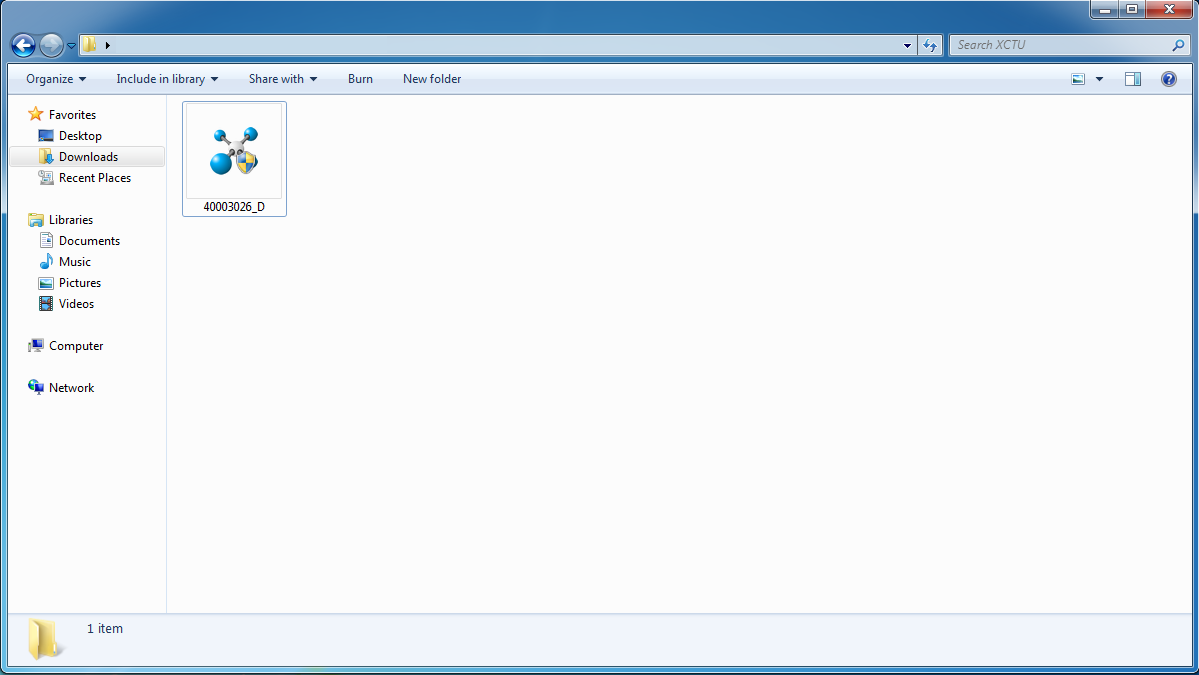
\includegraphics[width=0.8\linewidth]{Figures/XCTU/CarpetaDestino}}
\caption{Instalador del programa.}
\label{fig:Dest}
\end{figure}

Al ejecutar dicho archivo, el instalador mostrará la pantalla de bienvenida como se muestra en la figura \ref{fig:HXctu} de la página \pageref{fig:HXctu}. Pulse el botón \textit{\textbf{Next}}.

\begin{figure}[H] % Example image
\center{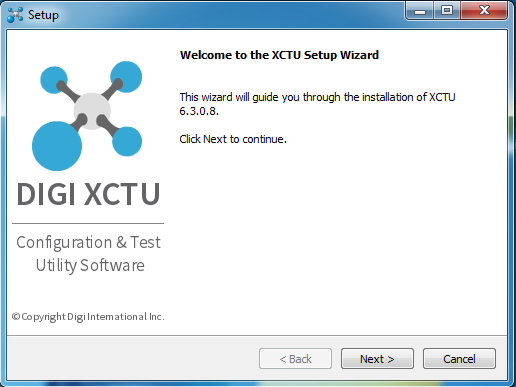
\includegraphics[width=0.65\linewidth]{Figures/XCTU/BienvenidaInstalador}}
\caption{Ventana principal del instalador de XCTU.}
\label{fig:HXctu}
\end{figure}

Se presentarán al usuario los términos y condiciones de uso del software, mismos que deberán ser aceptados para continuar utilizando el software. Tras ello, dar clic en el botón \textit{\textbf{Next}}. En la siguiente ventana, el usuario deberá indicar la carpeta donde el software se instalará, como se muestra en la figura \ref{fig:DirIn} dar clic en el botón \textit{\textbf{Next}}.

\begin{figure}[H] % Example image
\center{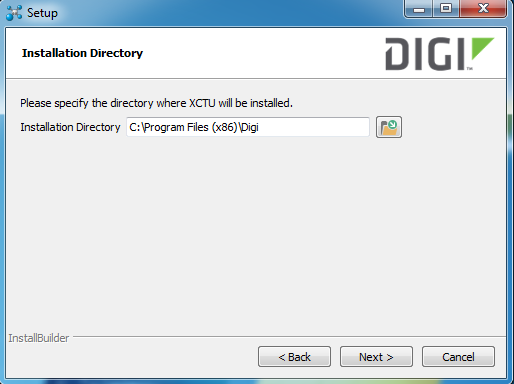
\includegraphics[width=0.65\linewidth]{Figures/XCTU/Direccion}}
\caption{Carpeta de destino de la instalación.}
\label{fig:DirIn}
\end{figure}

La copia de archivos tendrá lugar y habrá que esperar a que la misma termine, siendo la ventana del instalador quien se actualizará mostrando el progreso y después el aviso de que ha terminado. Una vez que dicho aviso aparezca, dar clic en el botón \textit{\textbf{Next}}. El proceso de instalación habrá terminado con una ventana como la de la figura \ref{fig:InstEnd} y solo resta dar clic en el botón \textit{\textbf{Finish}}.

\begin{figure}[H] % Example image
\center{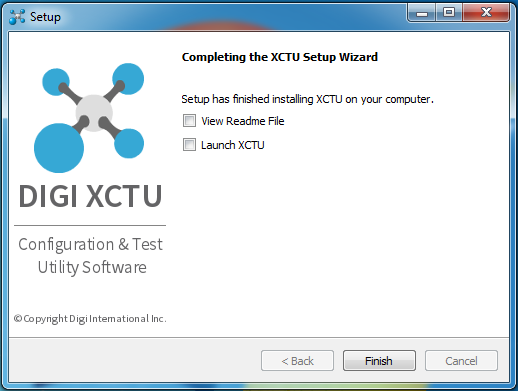
\includegraphics[width=0.65\linewidth]{Figures/XCTU/Finalizacion}}
\caption{El instalador informa que el proceso ha terminado correctamente.}
\label{fig:InstEnd}
\end{figure}
%---------------------------------------------------

\subsection{Apertura del programa}\label{subsec:exe}

El software estará disponible para su ejecución siguiendo la siguiente ruta: Menú Inicio $>$ Todos los programas $>$ Digi $>$ XCTU $>$ XCTU.exe, como se muestra en la figura \ref{fig:StartXC} de la página \pageref{fig:StartXC}.

\begin{figure}[H] % Example image
\center{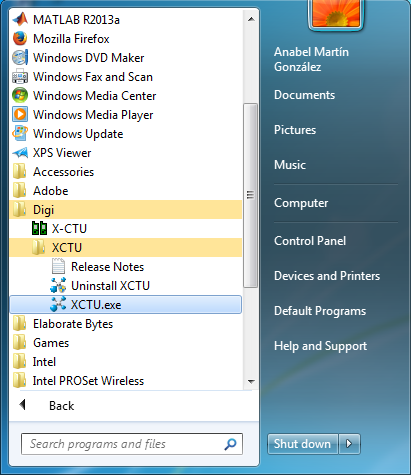
\includegraphics[width=0.5\linewidth]{Figures/XCTU/Inicioprograma}}
\caption{Archivo de inicio del software XCTU.}
\label{fig:StartXC}
\end{figure}

El programa cargará los archivos necesarios hasta desplegar la ventana principal del software, mostrado en la figura \ref{fig:Home}.

\begin{figure}[H] % Example image
\center{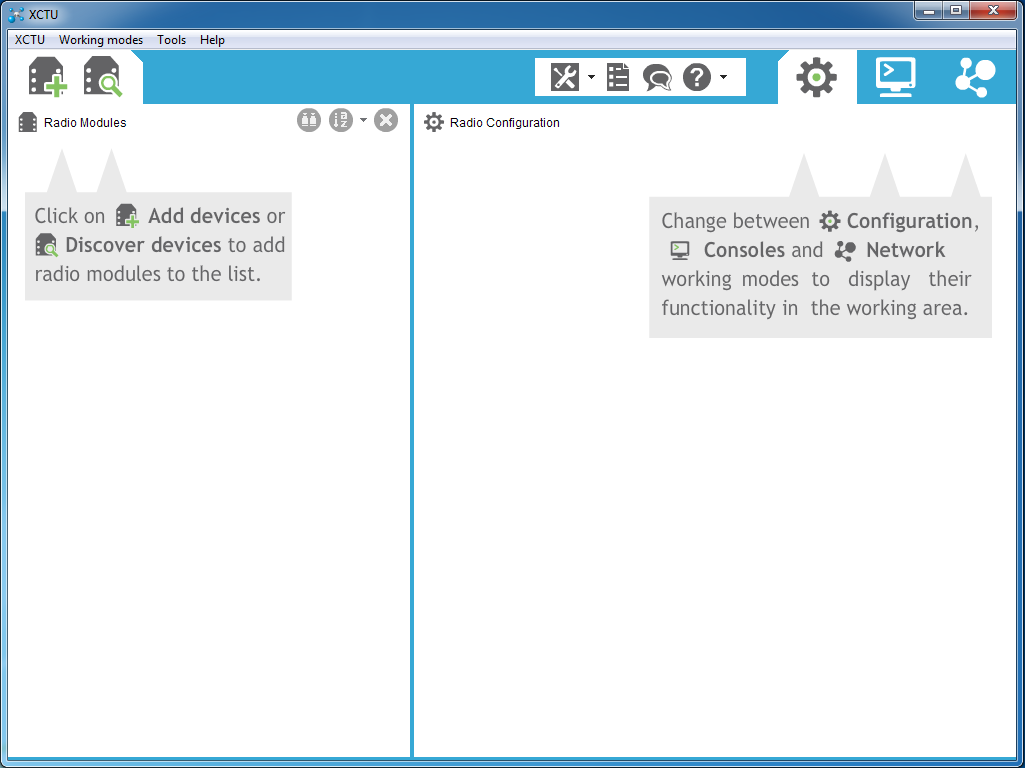
\includegraphics[width=0.6\linewidth]{Figures/XCTU/Home}}
\caption{Ventana principal de XCTU.}
\label{fig:Home}
\end{figure}

\section{Conexión y programación de los XBEE} 
Para conectar los XBEE a la PC, es necesario contar con un dispositivo que permita la comunicación serial mediante puertos USB, como el que se muestra en la figura \ref{fig:Board}. Existen distintos modelos en el mercado que varían en precio como en diseño, pero al final la funcionalidad es la misma. El XBEE deberá ser colocado con cuidado sobre la placa. 

\begin{figure}[H] % Example image
\center{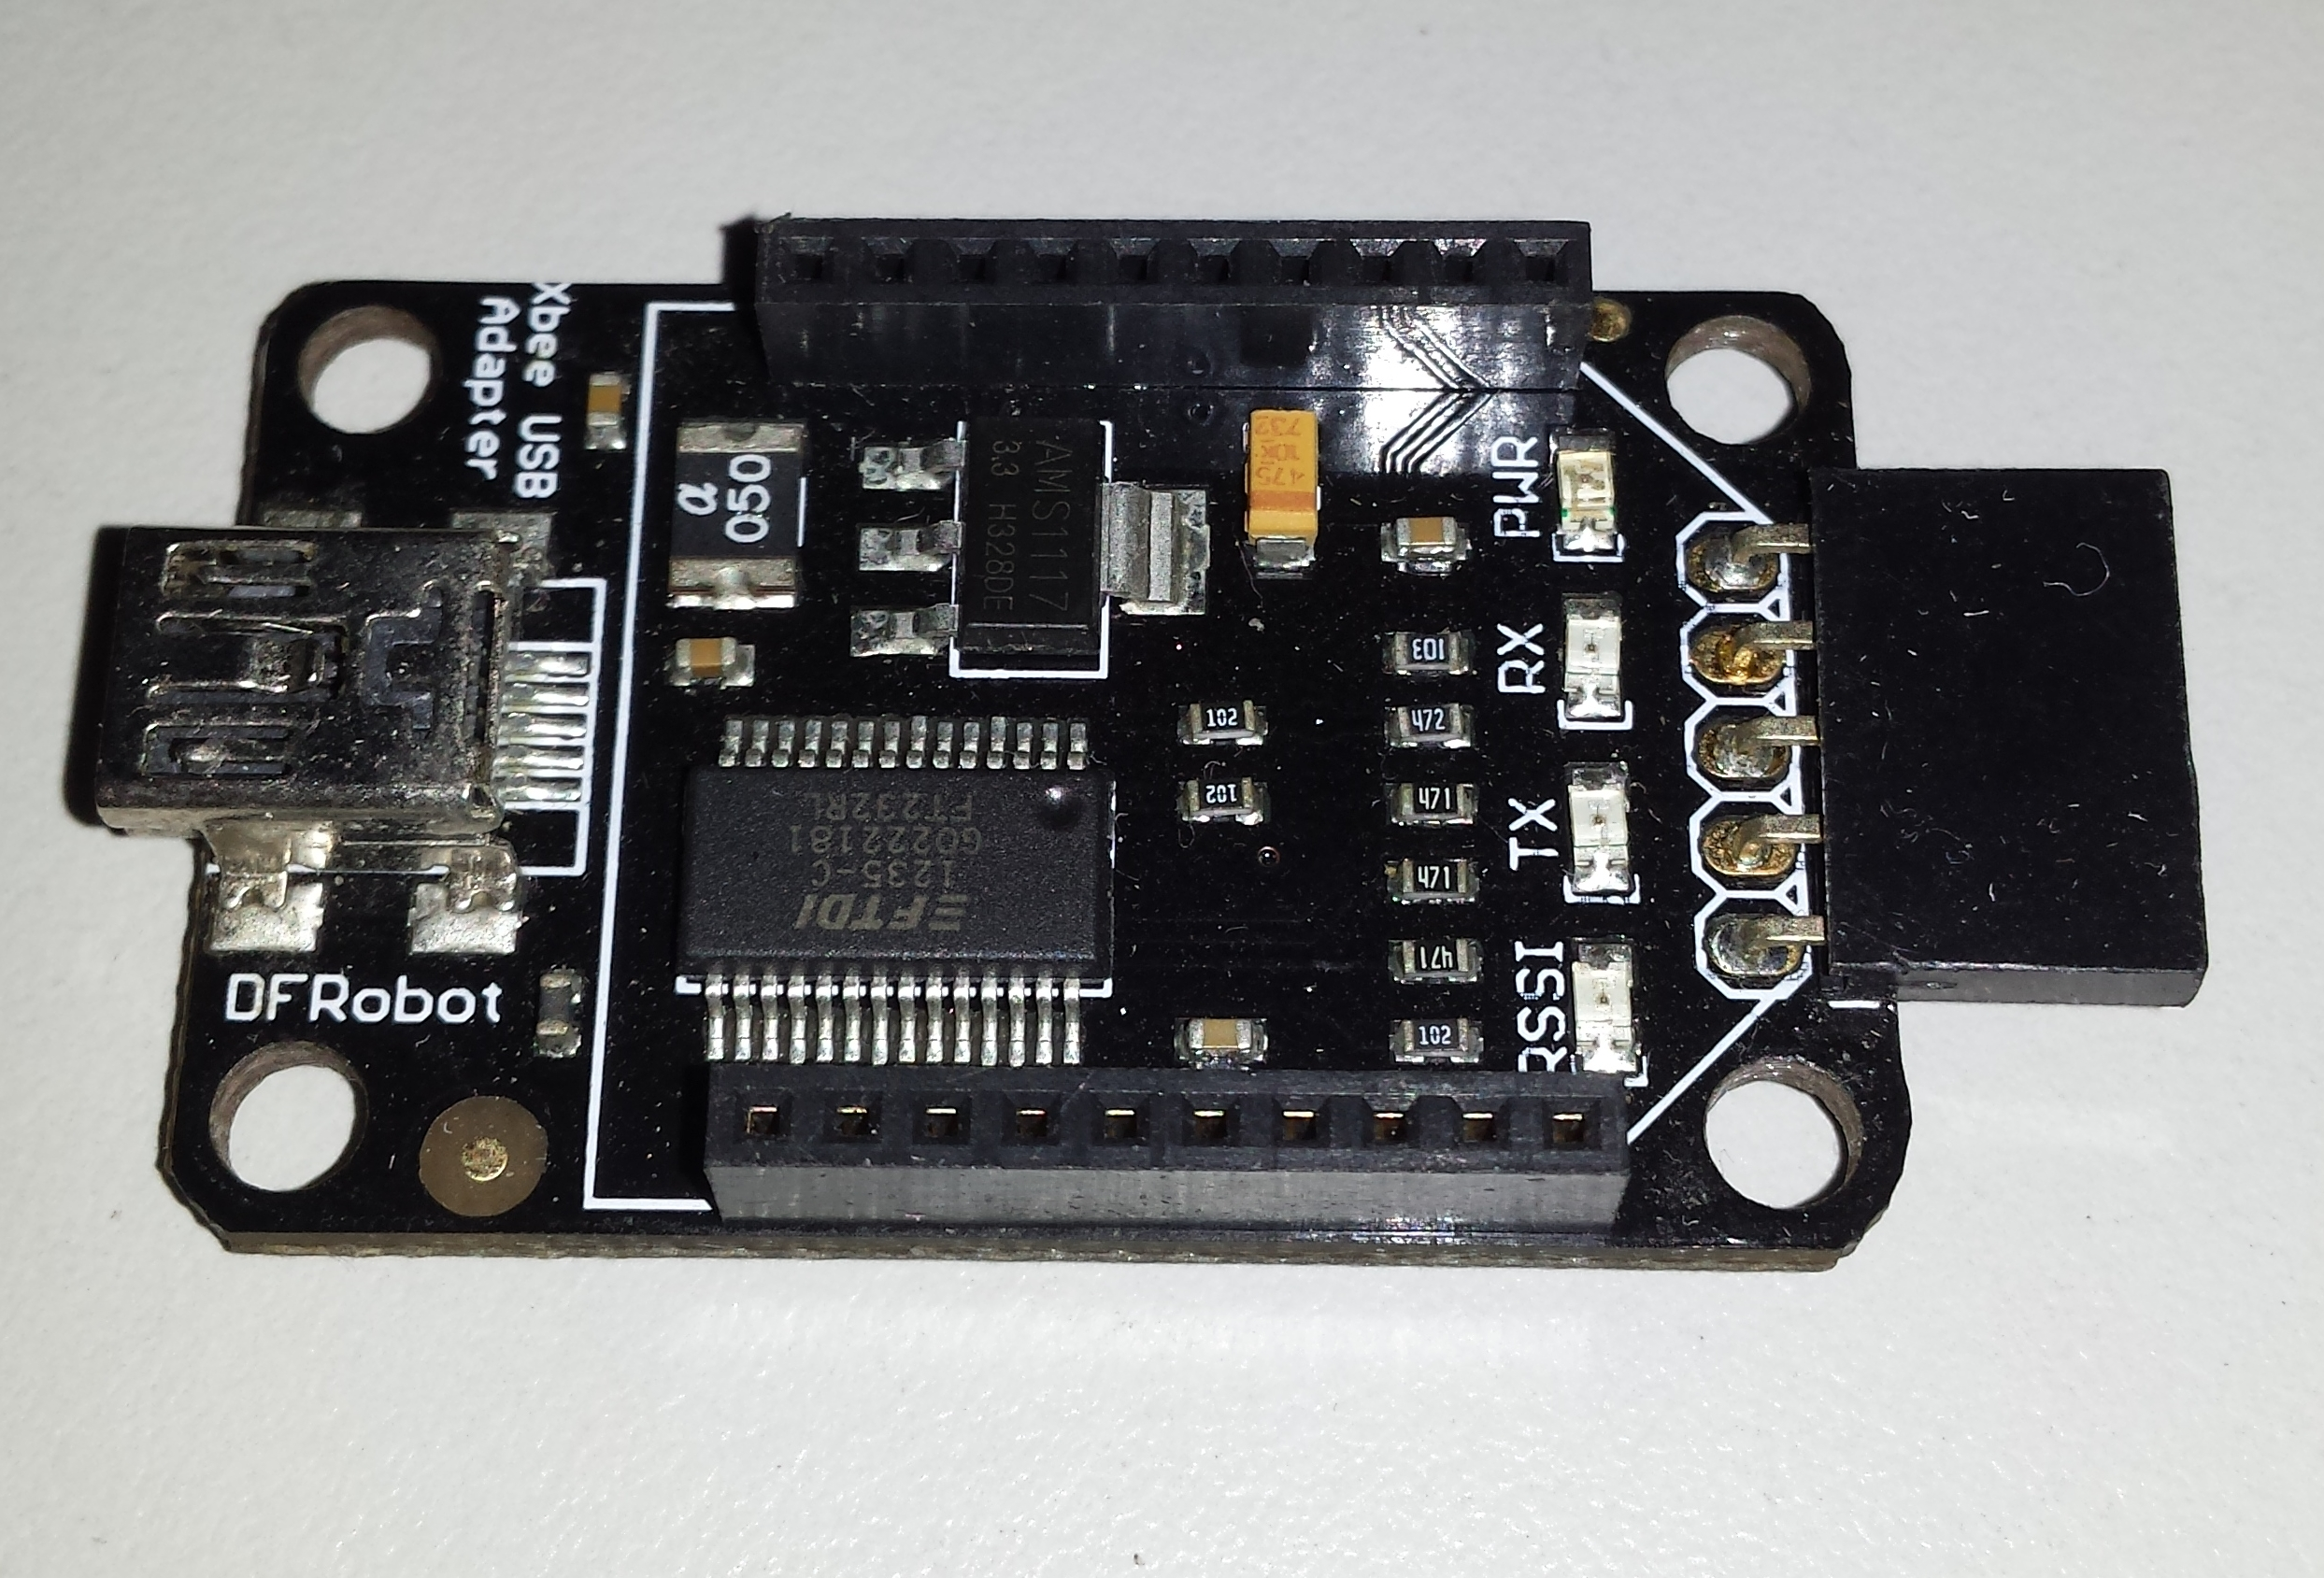
\includegraphics[width=0.74\linewidth]{Figures/XCTU/Board}}
\caption{Dispositivo que permite comunicación entre el XBEE y la PC.}
\label{fig:Board}
\end{figure}

Al conectarle con el cable a la PC, el sistema operativo comenzará con la instalación de los controladores necesarios, desplegando una ventana como la que se muestra en la figura \ref{fig:VentanaDeDrivers} una vez sea realizada con éxito.

\begin{figure}[H] % Example image
\center{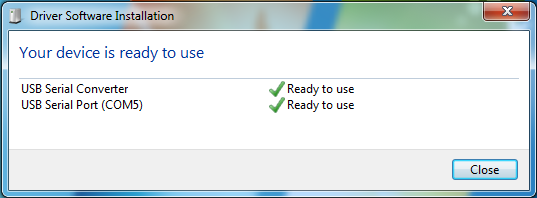
\includegraphics[width=0.74\linewidth]{Figures/XCTU/DrvsOk}}
\caption{Ventana que indica una correcta instalación de drivers.}
\label{fig:VentanaDeDrivers}
\end{figure}

En caso de que la ventana muestre que Windows no encontró los drivers, será necesario que se refiera a la sección \ref{subsec:Error}. En otro caso, puede saltarse esta guía hasta la sección \ref{subsec:Fine}.
%------------------------------------------------

\subsection{Instalación de controladores}\label{subsec:Error} % Sub-section
\subsubsection{Requerimientos para la instalación}
Si la ventana de instalación de drivers despliega el siguiente mensaje: "\textit{FT232R USB UART \ \ \ \ No driver found}", entonces debe visitar la página web de \href{http://www.ftdichip.com/Drivers/VCP.htm}{FTDI CHIP}\footnotemark, que contiene una tabla como la que se muestra en la figura \ref{fig:TablaCont}.

\footnotetext{http://www.ftdichip.com/Drivers/VCP.htm}

\begin{figure}[H] % Example image
\center{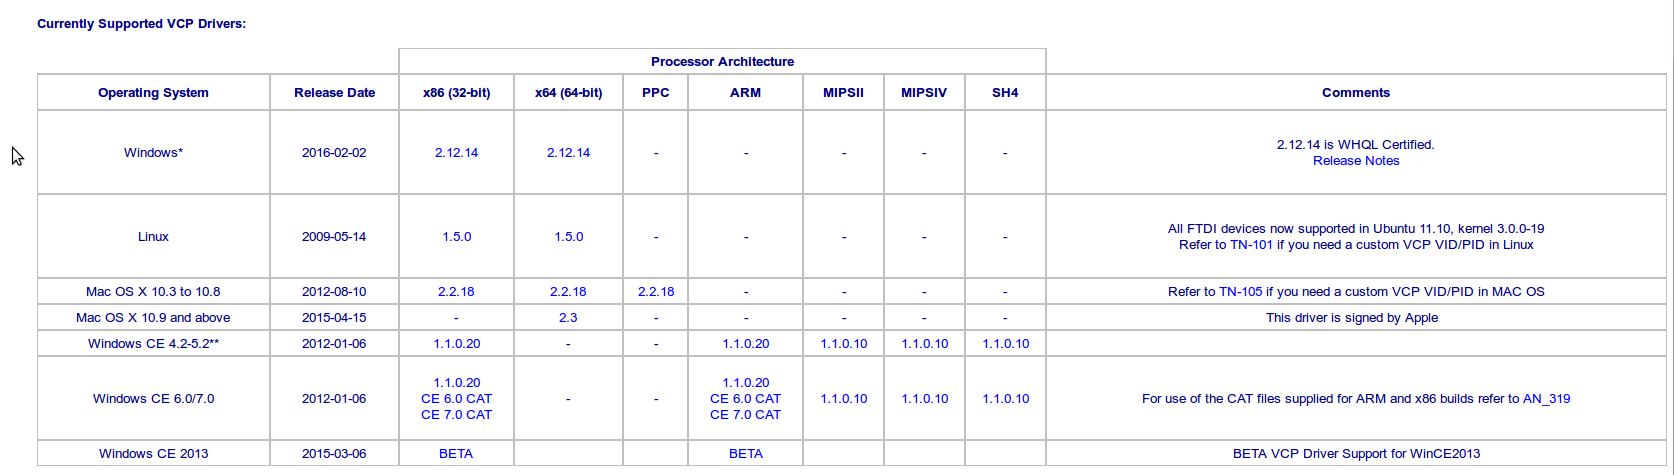
\includegraphics[width=0.74\linewidth]{Figures/XCTU/tablaftdi}}
\caption{Tabla de controladores.}
\label{fig:TablaCont}
\end{figure}

Se seleccionará el link correspondiente a la celda cuyos encabezados indiquen sus correspondientes sistema operativo y arquitectura. Se iniciará un proceso de descarga. Es necesario conocer el directorio donde estarán ubicados estos archivos, dado que deberán ser descomprimidos y luego indicados explícitamente en un asistente de Windows. Ahora, deberá abrir el \textbf{\textit{Menú Start}}, dar clic derecho a \textbf{\textit{Computer}} y seleccionar \textbf{\textit{Manage}}, como se indica en la figura \ref{fig:Man1} de la página \pageref{fig:Man1}. Este último paso requiere permisos de administrador. Si usted no los posee, contacte con el administrador del sistema.

\begin{figure}[H] % Example image
\center{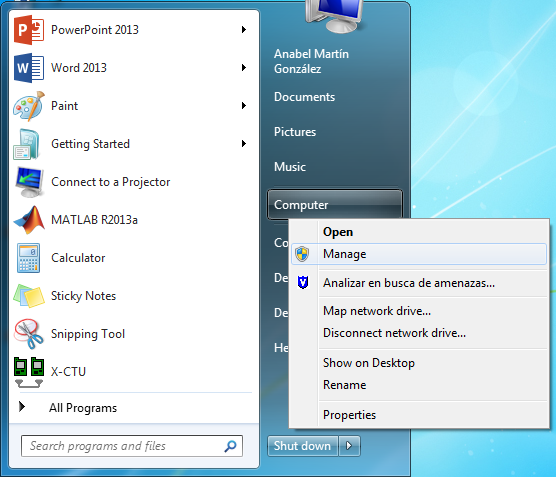
\includegraphics[width=0.6\linewidth]{Figures/XCTU/Manage}}
\caption{Ubicación del administrador de dispositivos.}
\label{fig:Man1}
\end{figure}

Se abrirá una ventana. En el listado del lado izquierdo, seleccionar \textit{\textbf{Device Manager}}, entonces la pantalla se mostrará como indica la figura \ref{fig:DevMan}.

\begin{figure}[H] % Example image
\center{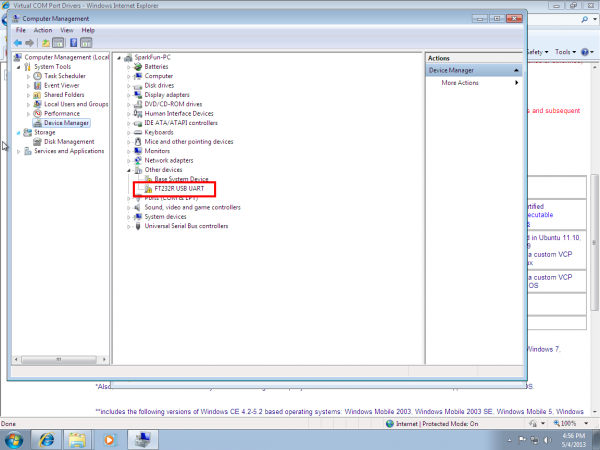
\includegraphics[width=0.6\linewidth]{Figures/XCTU/DeviceMngr}}
\caption[Administrador de Dispositivos]{Administrador de Dispositivos. Imagen tomada de \href{https://learn.sparkfun.com/tutorials/how-to-install-ftdi-drivers/all}{Sparkfun}.\footnotemark}
\label{fig:DevMan}
\end{figure}

\footnotetext{https://learn.sparkfun.com/tutorials/how-to-install-ftdi-drivers/all. A partir de aquí, el resto de las figuras de la sección \ref{subsec:Error} serán tomadas de dicha web salvo que se indique lo contrario.}

\subsubsection{Instalación}\label{subsubsec:loop}

Debe encontrar el dispositivo cuyo controlador no pudo ser instalado (\textit{FT232R USB UART}) en la sección de \textit{Other devices}, por lo que se deberá dar clic derecho en él y seleccionar la opción \textit{\textbf{Update Driver Software}}, como indica la figura \ref{fig:DevMan2}.\label{subsec:st}

\begin{figure}[H] % Example image
\center{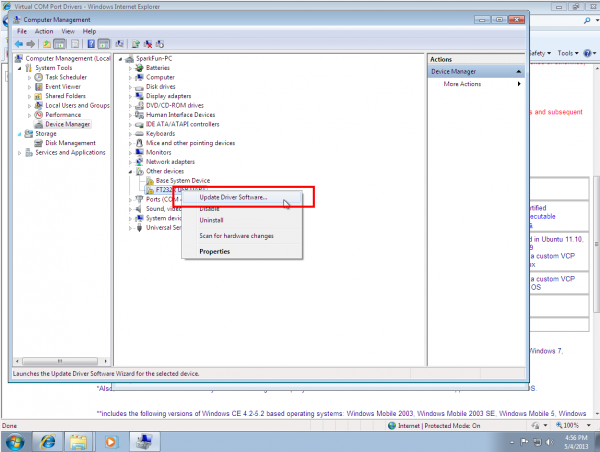
\includegraphics[width=0.9\linewidth]{Figures/XCTU/DeviceMngr2}}
\caption{Actualizar controlador.}
\label{fig:DevMan2}
\end{figure}

La ventana que ahora aparece es el asistente de instalación de los controladores descargados en la tabla de la figura \ref{fig:TablaCont}. Seleccionar \textit{\textbf{Browse my computer for driver software}}, como se indica en la figura \ref{fig:Asis} de la página \pageref{fig:Asis}.

\begin{figure}[H] % Example image
\center{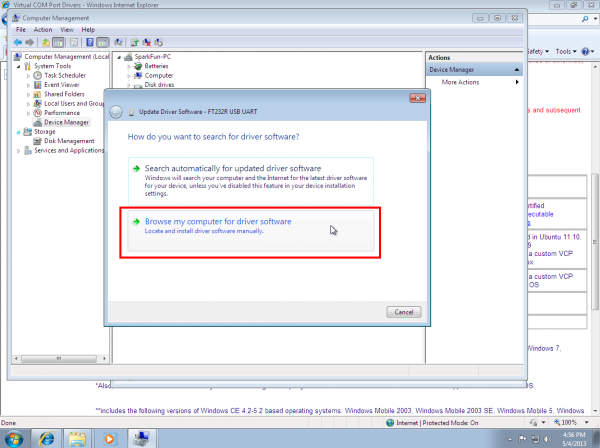
\includegraphics[width=0.6\linewidth]{Figures/XCTU/DeviceMngr3}}
\caption{Asistente de instalación del controlador.}
\label{fig:Asis}
\end{figure}

Es entonces en la ventana que ahora debe mostrarse, que se accederá a la carpeta que se creó tras descomprimir la descarga del controlador. Se hará dando clic al botón \textbf{\textit{Browse}} y se navegará hasta seleccionarla en la ventana emergente. Clic en \textit{\textbf{OK}}, como se muestra en la figura \ref{fig:Asis2}.  

\begin{figure}[H] % Example image
\center{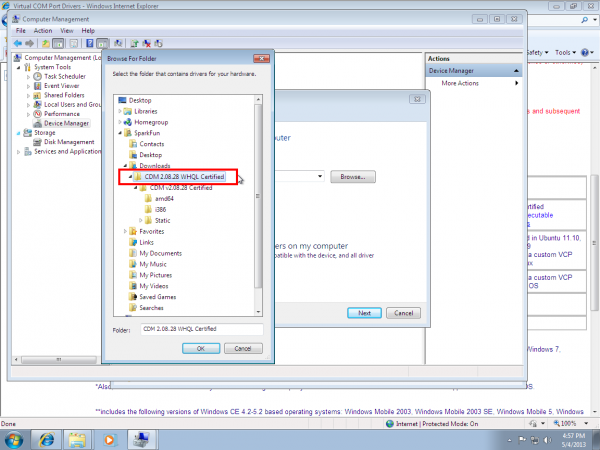
\includegraphics[width=0.6\linewidth]{Figures/XCTU/DeviceMngr4}}
\caption{Carpeta del controlador.}
\label{fig:Asis2}
\end{figure}

Verifique también que la opción \textit{Include subfolders} esté palomeada como en la figura \ref{fig:Subf} de la página \pageref{fig:Subf}, y dar clic al botón \textit{\textbf{Next}}. 

\begin{figure}[H] % Example image
\center{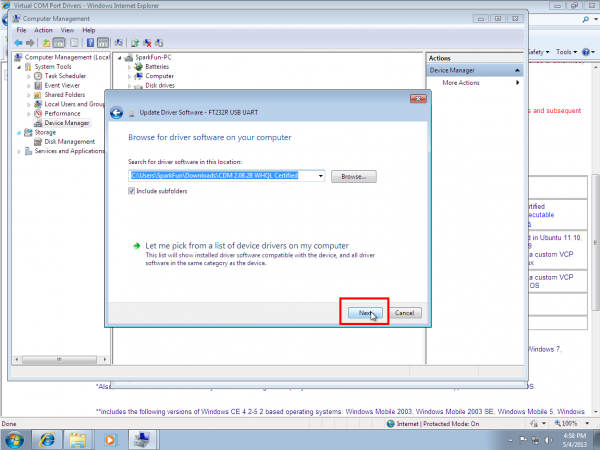
\includegraphics[width=0.66\linewidth]{Figures/XCTU/DeviceMngr5}}
\caption{Selección de carpeta.}
\label{fig:Subf}
\end{figure}

Tras un proceso que tomará algunos segundos, se mostrará una ventana de éxito en la instalación, tal y como se ve en la figura \ref{fig:Inst1}, y el asistente podrá cerrarse.

\begin{figure}[H] % Example image
\center{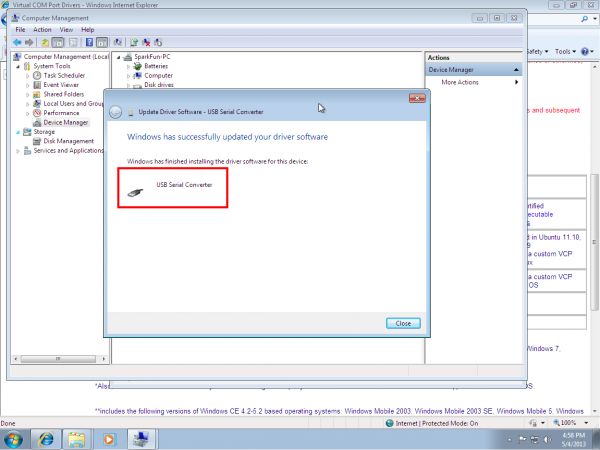
\includegraphics[width=0.63\linewidth]{Figures/XCTU/DeviceMngr6}}
\caption{Instalación exitosa.}
\label{fig:Inst1}
\end{figure}

Sin embargo, la instalación aún no está terminada, por lo que el proceso deberá repetirse desde el inicio de esta subsección \ref{subsubsec:loop}, pero ahora, en vez de actualizar el driver de \textit{FT232R USB UART}, se hará con el de \textit{\textbf{USB Serial Port}}, como se observa en la figura \ref{fig:Inst2} usando nuevamente la misma carpeta de controladores que antes se descomprimió.

\begin{figure}[H] % Example image
\center{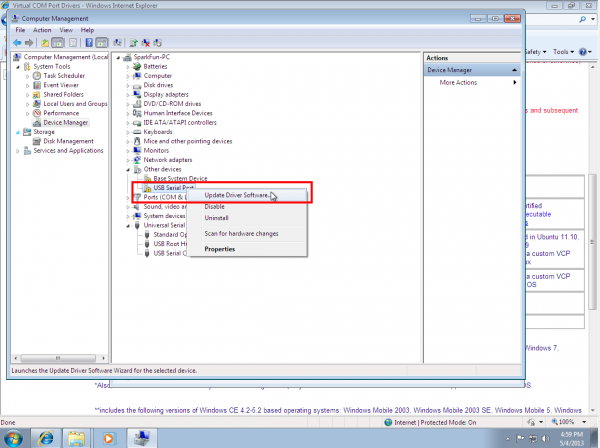
\includegraphics[width=0.63\linewidth]{Figures/XCTU/DeviceMngr7}}
\caption{Segunda instalación.}
\label{fig:Inst2}
\end{figure}

Al finalizar, se mostrará un dispositivo conectado como un puerto serial y el número asignado al mismo, como se muestra en la figura \ref{fig:Success}. Tomar nota del número de puerto asignado al XBEE.

\begin{figure}[H] % Example image
\center{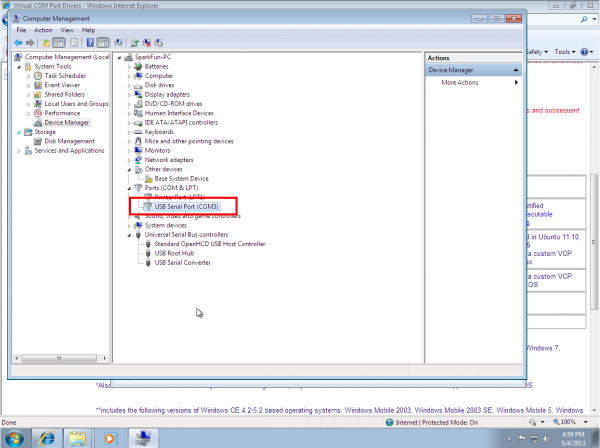
\includegraphics[width=0.63\linewidth]{Figures/XCTU/DeviceMngr8}}
\caption{Instalación exitosa de los controladores.}
\label{fig:Success}
\end{figure}

No será necesario repetir esta subsección \ref{subsec:Error} cada que un XBEE se conecte, ya que a partir de ahora, todos los dispositivos XBEE serán reconocidos automáticamente como una interfaz serial.

Este proceso de instalación fue tomado de los tutoriales de \href{https://learn.sparkfun.com/tutorials/how-to-install-ftdi-drivers/all}{Sparkfun}\footnotemark.

\footnotetext{https://learn.sparkfun.com/tutorials/how-to-install-ftdi-drivers/all con último acceso el 3 de Febrero de 2016}
%------------------------------------------------

\subsection{Reconocimiento del XBEE con XCTU}\label{subsec:Fine}
\subsubsection{Identificación del puerto}\label{subsubsec:Iden}
Ante todo, es necesario reconocer mediante qué puerto un XBEE está conectado a la PC. Por lo tanto, se deberán, seguir los siguientes pasos: abrir el \textit{\textbf{menú Start}}, clic derecho en \textit{\textbf{Computer}}, clic en \textit{\textbf{Manage}}, tal y como se muestra en la figura \ref{fig:Man}. Se requieren permisos de administrador para acceder a esta ventana.

\begin{figure}[H] % Example image
\center{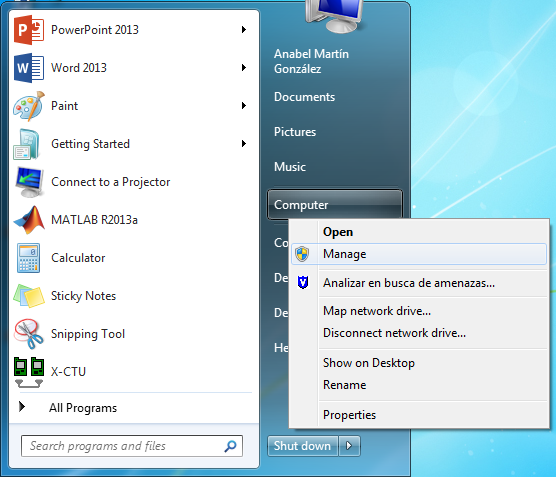
\includegraphics[width=0.63\linewidth]{Figures/XCTU/Manage}}
\caption{Ubicación del administrador de dispositivos.}
\label{fig:Man}
\end{figure}

En la ventana que se abre, en el menú de la izquierda, dar clic a \textit{\textbf{Device Manager}}, tal como se observa en la figura \ref{fig:DevM} de la página \pageref{fig:DevM}. 

\begin{figure}[H] % Example image
\center{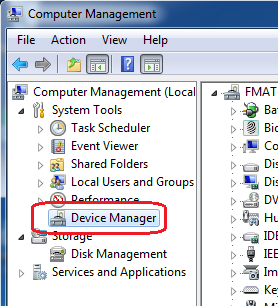
\includegraphics[width=0.5\linewidth]{Figures/XCTU/DeviceMan}}
\caption{Localización del Device Manager.}
\label{fig:DevM}
\end{figure}

Entonces, ubicar el menú desplegable \textit{Ports (COM \& LPT)}, y ahí debe indicarse el número de puerto utilizado, como se indica en la figura \ref{fig:IdCom}.

\begin{figure}[H] % Example image
\center{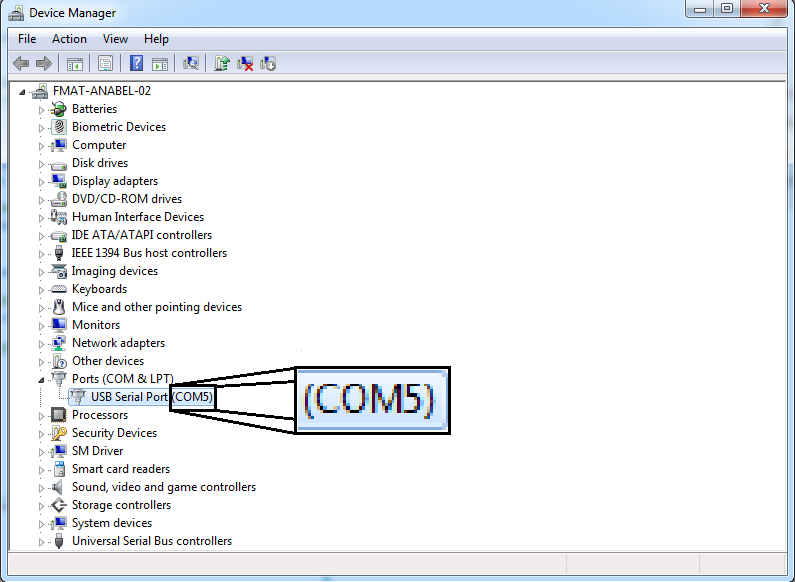
\includegraphics[width=0.7\linewidth]{Figures/XCTU/IdentificarCOM}}
\caption{Identificador del puerto COM utilizado por el XBEE.}
\label{fig:IdCom}
\end{figure}

\subsubsection{Añadir XBEE a XCTU}

\begin{wrapfigure}{r}{0.25\textwidth} %this figure will be at the right
    \centering
    
\includegraphics[width=0.10\textwidth]{Figures/XCTU/AddDeviceButton}
    \caption{Botón para añadir un dispositivo.}
    \label{fig:AddDevice}
\end{wrapfigure}

Se debe abrir el software XCTU (mire la subsección \ref{subsec:exe}). Una vez en la ventana principal, se debe ubicar el botón para añadir un dispositivo, que es como se muestra en la figura \ref{fig:AddDevice}, que se encuentra en la parte superior izquierda de la ventana del programa.

Tras darle clic, se abrirá una ventana como la que se muestra en la figura \ref{fig:AddW}. En esta ventana se observa una sección donde se debe de indicar el puerto al que el XBEE está conectado, y otra donde se pide especificar ciertos valores de la conexión, y dar clic al botón \textit{\textbf{Finish}}. Si el XBEE es nuevo, se recomienda utilizar los valores por defecto de esta ventana, y de ser el caso, indicar explícitamente en la casilla que el dispositivo es programable.

\begin{figure}[H] % Example image
\center{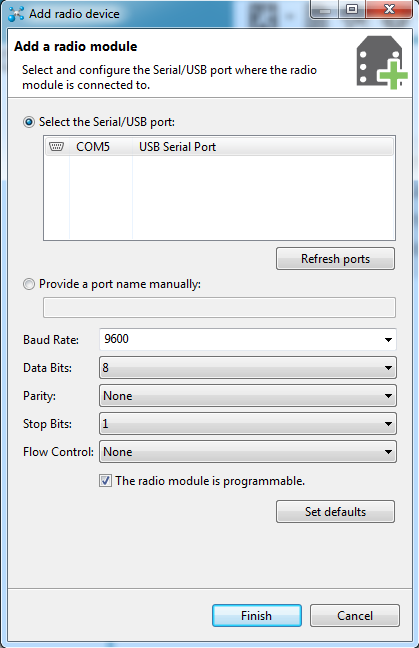
\includegraphics[width=0.45\linewidth]{Figures/XCTU/AddDeviceW}}
\caption{Ventana donde se especifica la conexión al dispositivo.}
\label{fig:AddW}
\end{figure}

En caso de que tras seguir los pasos del párrafo anterior el dispositivo aún no sea detectado, entonces utilice el botón para descubrir dispositivos conectados, como el que muestra la figura \ref{fig:SearchDev}. La función que realiza es muestrear el puerto a distintas configuraciones hasta entablar una conexión exitosa con el XBEE.

\begin{wrapfigure}{l}{0.25\textwidth} %this figure will be at the left
    \centering
    
\includegraphics[width=0.10\textwidth]{Figures/XCTU/SearchDevice}
    \caption{Botón para buscar un dispositivo.}
    \label{fig:SearchDev}
\end{wrapfigure}

Por tanto, al dar clic a dicho botón, se abre una ventana preguntando por el número de puerto a muestrear, como se indica en la figura \ref{fig:PS}. Se pueden escoger múltiples puertos en el caso de que dos o más XBEE estén conectados para que el sistema les descubra y se conozcan sus configuraciones de interfaz serial. Se sugiere escribir y marcar de forma visible a los dispositivos con su configuración (baud rate, bits de parada, etc.) para que sea más sencillo identificarles y añadirles al software XCTU mediante la herramienta de añadir dispositivo de la figura \ref{fig:AddW} de la página \pageref{fig:AddW}. Indique el puerto y de clic al botón \textit{\textbf{Next}}.

\begin{figure}[H] % Example image
\center{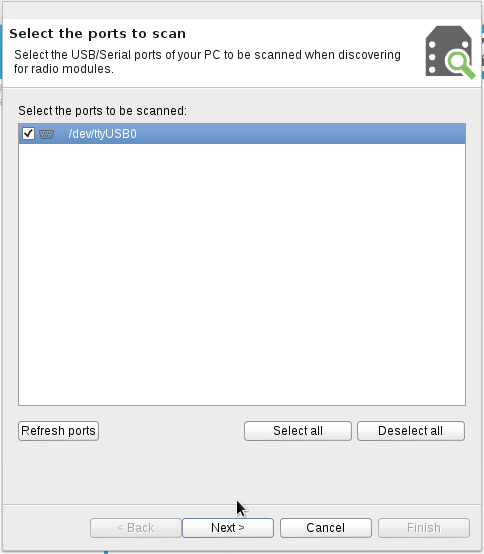
\includegraphics[width=0.45\linewidth]{Figures/XCTU/PortSearch}}
\caption{Indique el puerto que el programa muestreará.}
\label{fig:PS}
\end{figure}

Se abrirá una segunda ventana donde se pueden indicar varias configuraciones a evaluar, como el de la figura \ref{fig:PSe} de la página \pageref{fig:PSe}. En ella, se indica también el tiempo estimado que le tomará al software explorar a través de todas esas configuraciones. Si no se conoce ningún dato sobre el XBEE, puede marcar todas las opciones. De clic al botón \textit{\textbf{Finish}} para iniciar la búsqueda. Tomará varios minutos.

\begin{figure}[H] % Example image
\center{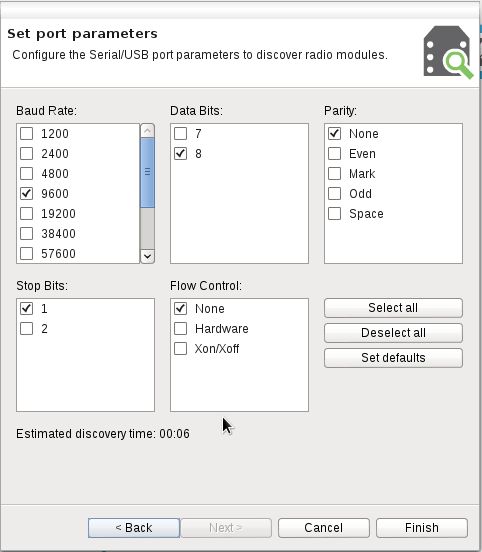
\includegraphics[width=0.45\linewidth]{Figures/XCTU/ParametrosSearch}}
\caption{Ventana de configuración de búsqueda.}
\label{fig:PSe}
\end{figure}

Una vez finalizada la búsqueda, otra ventana mostrará todos los XBEE detectados por el software, como se muestra la figura \ref{fig:DvF}. Seleccione todos los dispositivos que desea añadir al software XCTU y de clic al botón \textit{\textbf{Add selected devices}}.

\begin{figure}[H] % Example image
\center{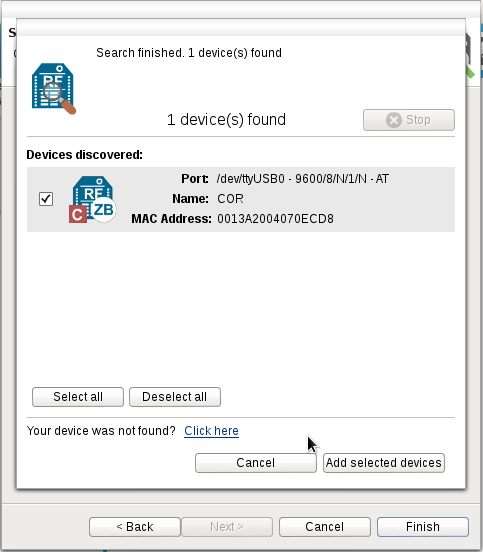
\includegraphics[width=0.37\linewidth]{Figures/XCTU/DeviceFound}}
\caption{Lista de XBEE encontrados por la herramienta de búsqueda.}
\label{fig:DvF}
\end{figure}

Tras cerrar todas las ventanas relacionadas con la búsqueda del dispositivo, se puede observar en la ventana principal de XCTU que, en la parte izquierda, se encuentra el XBEE descubierto y está listo para ser programado, como se observa en la figura \ref{fig:XCTM}.

\begin{figure}[H] % Example image
\center{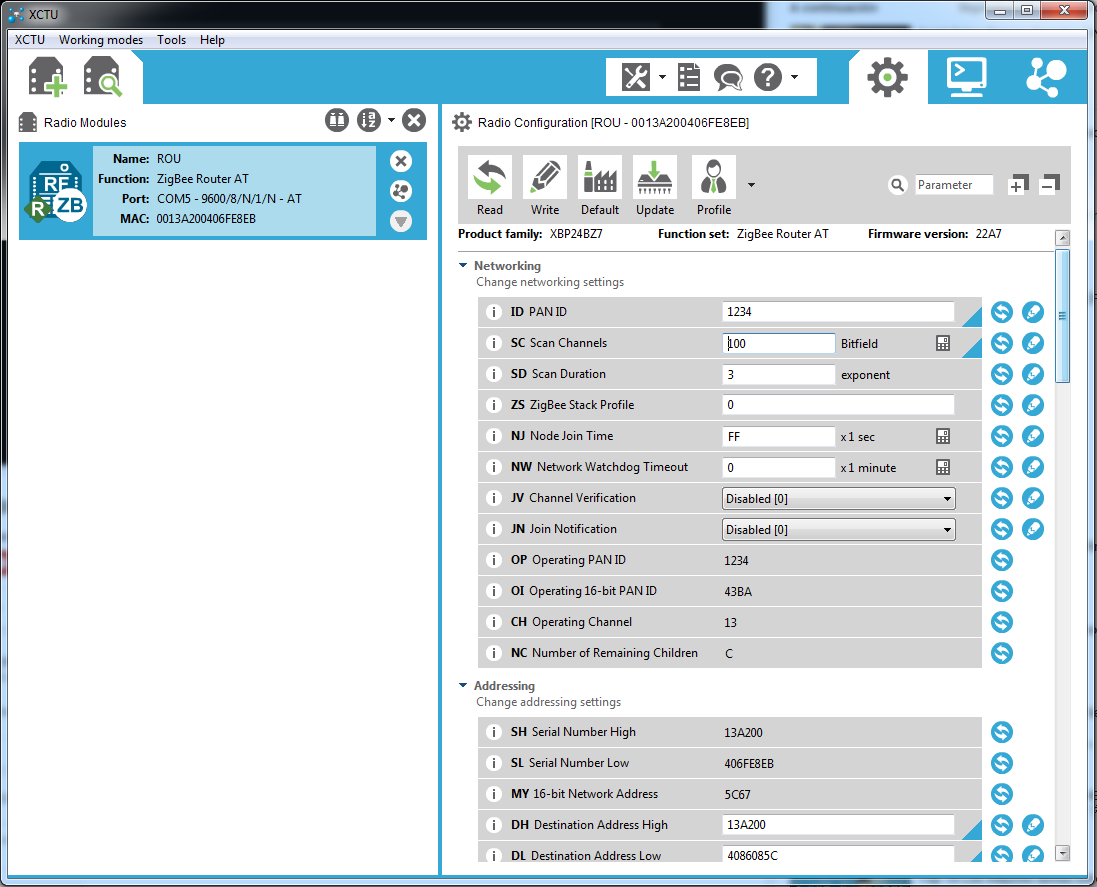
\includegraphics[width=0.7\linewidth]{Figures/XCTU/XCTUMain}}
\caption{Ventana principal de XCTU con un XBEE añadido.}
\label{fig:XCTM}
\end{figure}

\subsection{Programación del XBEE}
\subsubsection{Configurando los modos}\label{StartConf}
Una vez asociado por lo menos un XBEE a XCTU, como se observa en la figura \ref{fig:XCTM}, se puede comenzar con la configuración del mismo. En el lado izquierdo de la ventana, podrá ubicar una sección con algunos datos relacionados al XBEE que se encuentra conectado, como muestra la figura \ref{fig:RtrInf}. 

\begin{figure}[H] % Example image
\center{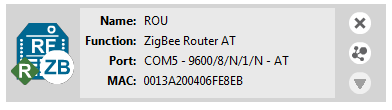
\includegraphics[width=0.7\linewidth]{Figures/XCTU/RouterInfo}}
\caption{Información del XBEE asociado a XCTU.}
\label{fig:RtrInf}
\end{figure}

Es importante que tenga en cuenta los dígitos del apartado \textbf{MAC}, ya que serán útiles en la posterior configuración de los dispositivos. Los primeros ocho dígitos serán conocidos como la \underline{parte alta} de la dirección física (en el caso de la figura \ref{fig:RtrInf} de la página \pageref{fig:RtrInf}, 0013A200), y los últimos ocho como la \underline{parte baja} de la dirección física (en la figura \ref{fig:RtrInf}, 406FE8EB).

Si se da clic en este apartado, XCTU leerá toda la configuración del XBEE para ser presentado al usuario. La información es separada mediante secciones y tablas, y se diferencian ligeramente dependiendo de la versión de firmware y el tipo de función programada. 

\begin{figure}[H] % Example image
\center{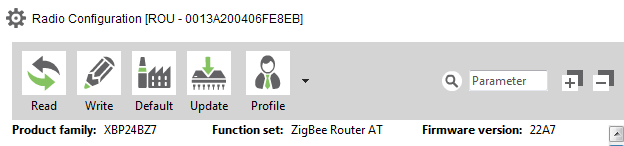
\includegraphics[width=0.7\linewidth]{Figures/XCTU/TopMain}}
\caption{Apartado de información y herramientas.}
\label{fig:TMain}
\end{figure}

En la parte superior de esta ventana, se halla un apartado como el de la figura \ref{fig:TMain}, que ofrece al usuario tanto herramientas así como información sobre el estado de la configuración del XBEE.

A continuación, una breve explicación de esta área:

\begin{itemize}
	\item \textbf{Read}: Se lee la configuración del XBEE y se muestran en las tablas. 
	\item \textbf{Write}: Se guardan y escriben al dispositivo todos los cambios realizados a los parámetros.
	\item \textbf{Default}: Restaura al XBEE a las configuraciones por defecto del firmware instalado.
	\item \textbf{Update}: Para cambiar la función asignada y la versión de firmware.
	\item \textbf{Profile}: Para guardar un conjunto de configuraciones en un archivo externo, o para leer uno y desplegarlo en las tablas.
	\item \textbf{Product family}: Muestra el modelo físico del hardware.
	\item \textbf{Function set}: Muestra su función asignada.
	\item \textbf{Firmware version}: Muestra el número de su última versión.
\end{itemize}

Para el propósito de tener una topología de tipo \textit{\textbf{Par}}, es necesario contar con un XBEE programado como \textit{ZigBee Router AT} o como \textit{ZigBee End Device AT}, y otro XBEE como un \textit{ZigBee Coordinator AT}. Para obtenerlos, se da clic al botón \textbf{Update}. Se abrirá una ventana como la de la figura \ref{fig:Upd}.

\begin{figure}[H] % Example image
\center{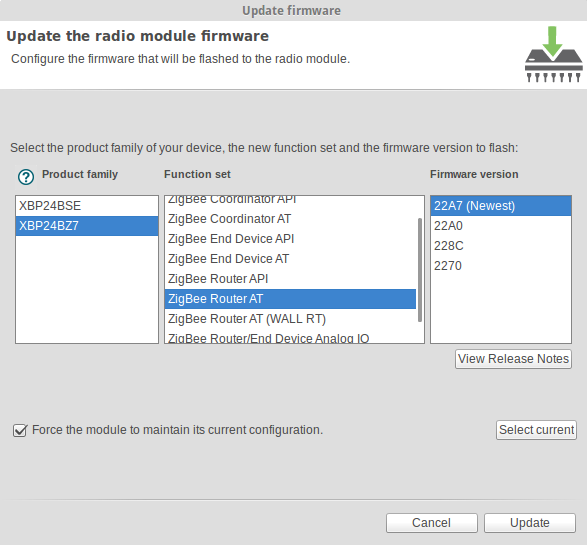
\includegraphics[width=0.7\linewidth]{Figures/XCTU/Update}}
\caption{Ventana de programación del firmware.}
\label{fig:Upd}
\end{figure}

En la lista del lado izquierdo, llamada \textit{Product family}, se seleccionará el modelo correspondiente al hardware que se tiene, es el mismo que se muestra en el área mostrada en la figura \ref{fig:TMain} de la página \pageref{fig:TMain}. En la segunda lista, llamada \textit{Function set}, se seleccionará el tipo de dispositivo. Se necesitan ya sea uno programado como ZigBee End Device AT o ZigBee Router AT, y un ZigBee Coordinator AT, así que se selecciona alguno de ellos (si el primer XBEE fue programado como End Device o Router, el segundo deberá ser un Coordinator, o viceversa). En la tercera lista, llamada \textit{Firmware version}, se selecciona alguno de la lista. El texto \textit{Newest} al lado de cierta versión, indica que es la más reciente y por tanto la más recomendada. Puede revisar las notas de los desarrolladores acerca de estas versiones en el botón \textbf{View Release Notes}. Si marca la opción \textit{Force the module to maintain its current configuration}, la nueva versión mantendrá configuraciones tales como el área de trabajo, sus identificadores, etc., por lo que se recomienda tenerla seleccionada. Se da clic al botón \textit{\textbf{Update}}. El asistente realizará el proceso de grabado de firmware y le tomará algunos minutos. Repita por cada XBEE a programar. Al terminar, podrá regresar a la ventana principal de XCTU para las últimas configuraciones.

\subsubsection{Configurando el Coordinador}
Los XBEE cuentan tanto con direcciones físicas, dadas por el fabricante y que son imposibles de cambiar, y de direcciones lógicas, que pueden ser configuradas de acuerdo a las necesidades del proyecto. Tenga en cuenta siempre la dirección física de los XBEE, ya que será necesario colocarlos en la configuración. En el coordinador, los parámetros a configurar son:

\begin{itemize}
	\item \textbf{ID} \textit{Personal Area Network ID o PAN ID} (identificador de red de área personal). 
	\item \textbf{OI} \textit{Operating 16-bit PAN ID} (identificador operativo de red de área personal de 16 bits).
	\item \textbf{CH} \textit{Operating Channel} (Canal operativo).
	\item \textbf{DH} \textit{Destination Address High} (Parte alta de la dirección de destino).
	\item \textbf{DL} \textit{Destination Address Low} (Parte baja de la dirección de destino).
\end{itemize}

Si dos terminales se encuentran en diferentes configuraciones (no aplica para las direcciones de destino), no serán capaces de encontrarse.

Para configurarlas, hay que introducir los siguientes datos en XCTU: 

En la sección \textit{Networking}:
\begin{itemize}
	\item[-] PAN ID: \texttt{\underline{1234}}.
	\item[-] Scan Channels: \texttt{\underline{100}}.
\end{itemize}

En la sección \textit{Addressing}:
\begin{itemize}
	\item[-] Destination Address High: [Parte \texttt{\underline{alta}} de la dirección física del 
	Router o End Device].
	\item[-] Destination Address Low: [Parte \texttt{\underline{baja}} de la dirección física del 
	Router o End Device].
\end{itemize}

Para terminar, de clic al botón \textit{\textbf{Write}} de la parte superior de la ventana.

\begin{wrapfigure}{l}{0.25\textwidth} %this figure will be at the left
    \centering
    
\includegraphics[width=0.10\textwidth]{Figures/XCTU/Console}
    \caption{Botón de inicio del modo terminal.}
    \label{fig:Term}
\end{wrapfigure}

\subsubsection{Configuración mediante comandos AT}\label{subsubsec:ConCoor}

A continuación, para programar el parámetro restante, es necesario ingresar al modo terminal. Para ello, se debe dar clic en el botón que se muestra en la figura \ref{fig:Term}. En el modo terminal o consola, se pueden enviar datos a otro XBEE y también se pueden leer datos recibidos de otro dispositivo, asi como entrar al modo de configuración mediante comandos AT (mire la figura \ref{fig:XTerm}), que es lo que a continuación se realizará.  

\begin{figure}[H] % Example image
\center{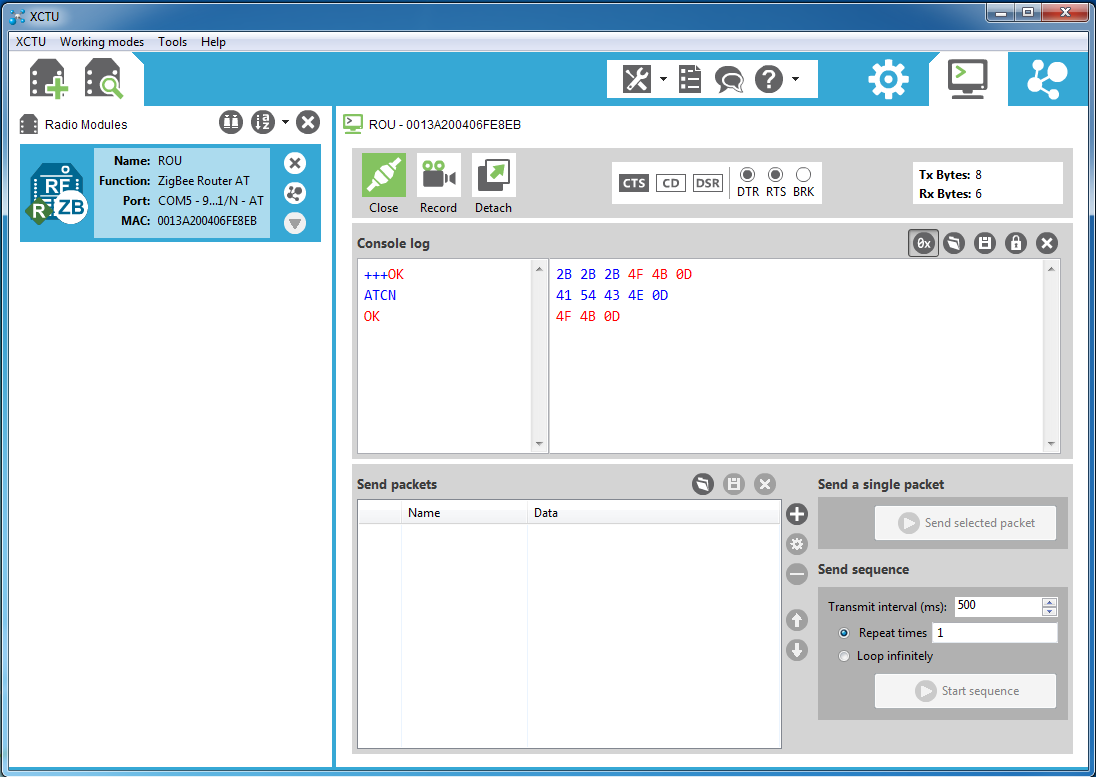
\includegraphics[width=0.7\linewidth]{Figures/XCTU/ConsoleWind}}
\caption{XCTU en modo consola.}
\label{fig:XTerm}
\end{figure}

Para iniciar con este modo, de clic al botón \textit{\textbf{Open}}, que es como el que se muestra en la figura \ref{fig:OpenC} de la página \pageref{fig:OpenC}. Esto habilitará la consola (\textit{Console log}), donde se podrá trabajar. En textos de color azul, se muestra lo que el usuario teclea en esta terminal. En textos de color rojo, se encuentran los datos recibidos del XBEE, que puede ser tanto respuesta de la comunicación con otro XBEE, así como respuesta del propio dispositivo conectado a la PC cuando se esté configurando.

\begin{wrapfigure}{r}{0.25\textwidth} %this figure will be at the left
    \centering
    
\includegraphics[width=0.10\textwidth]{Figures/XCTU/OpenButton}
    \caption{Botón de apertura de comunicación.}
    \label{fig:OpenC}
\end{wrapfigure}

En el recuadro blanco del lado izquierdo, teclee tres veces el caracter de suma (\textcolor{blue}{+++}). En color rojo, el XBEE deberá responder con un \textcolor{red}{OK}. Al recibir esta respuesta, el XBEE estará en modo de configuración por comandos AT\footnotemark. Ahora teclee el comando \textcolor{blue}{ATII 43BA}. El dispositivo deberá responder con otro mensaje de \textcolor{red}{OK}. Para confirmar que dicho valor fue establecido, teclee el comando \textcolor{blue}{ATII}. El XBEE deberá responder con el valor que le fue dicho explícitamente en la instrucción anterior: \textcolor{red}{43BA}. En otro caso, vuelva a indicárselo. Para finalizar, teclee el comando \textcolor{blue}{ATCN}. El XBEE responderá con un \textcolor{red}{OK}. Una vez que el dispositivo de esta última respuesta, retornará al modo de transmisión y recepción normal de datos. Es ahora que el Coordinador XBEE está configurado correctamente y está listo para ser utlizado. Cierre la comunicación de la terminal con el XBEE con el botón Close (quien sustituyó al botón Open de la figura \ref{fig:OpenC} en la misma posición). Los valores explícitamente proporcionados pueden modificarse para adecuarse a algún proyecto que lo requiriese, para ello, lea el manual que Digi u otros autores ofrecen sobre la programación de estos dispositivos.

\begin{wrapfigure}{l}{0.25\textwidth} %this figure will be at the left
    \centering
    
\includegraphics[width=0.10\textwidth]{Figures/XCTU/ConfMode}
    \caption{Botón de modo de configuración gráfico.}
    \label{fig:ConMode}
\end{wrapfigure}

Debe regresar al modo en que se configuraba todo de forma gráfica, para ello, de clic al botón que se muestra en la figura \ref{fig:ConMode}, que se ubica en la parte superior derecha de la ventana.

Para actualizar todas las configuraciones que se muestran, de clic al botón \textit{\textbf{Read}} que se encuentra en las herramientas de la parte superior de la ventana. Al final, las configuraciones deben aparecer como que se muestra en la figura \ref{fig:CoordAll} de la página \pageref{fig:CoordAll}.

\footnotetext{Si a mitad del proceso de configuración por comandos AT el XBEE deja de dar respuestas, es porque muy probablemente haya pasado un tiempo sin recibir comandos, por lo que el XBEE retornará a su estado de transmisión y recepción. Deberá volver a iniciar el modo de configuración por comandos AT con los tres caracteres de suma e iniciar el proceso de nuevo.}

\begin{figure}[H] % Example image
\center{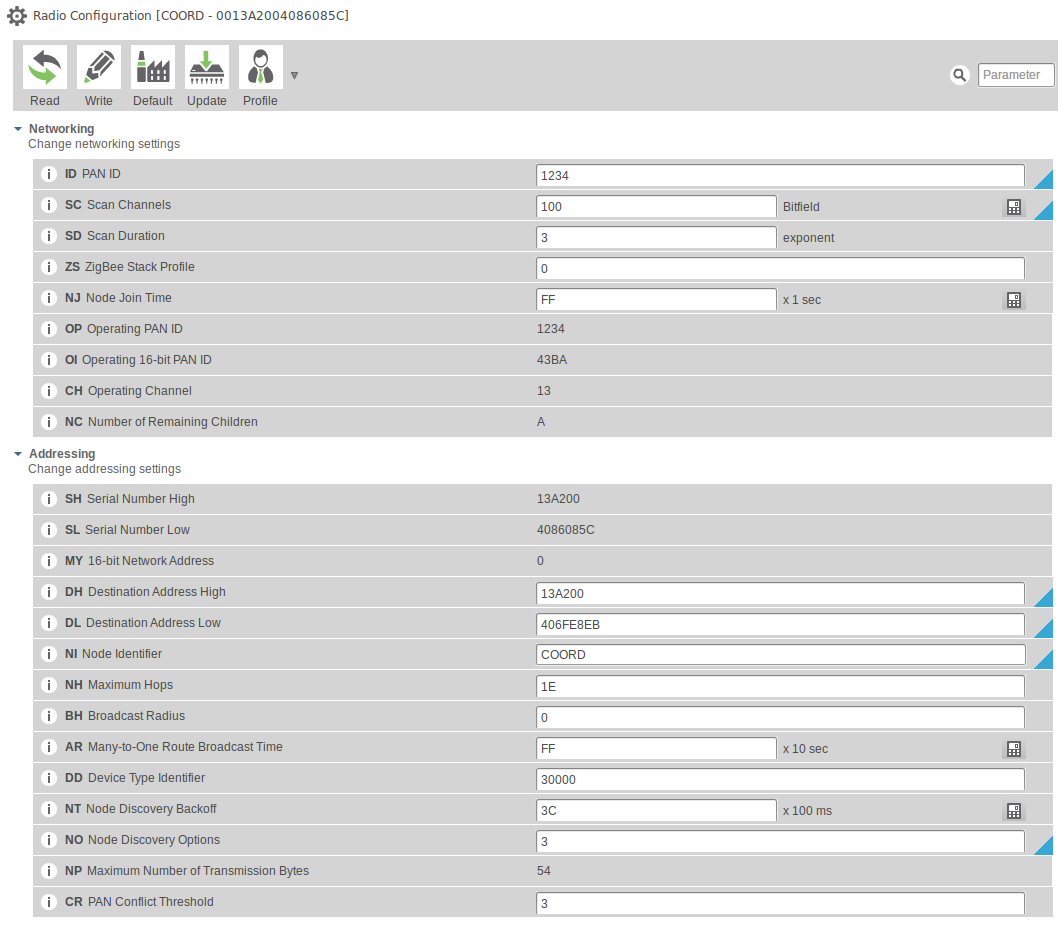
\includegraphics[width=0.9\linewidth]{Figures/XCTU/CoordConfAll}}
\caption{Configuraciones finales en el Coordinador.}
\label{fig:CoordAll}
\end{figure}

Tras verificar que todo esté debidamente configurado, se procede a realizar lo propio con el dispositivo Router o End Device. Para efectos de esta guía, se usará un Router.

\subsubsection{Configurando el Router}
La configuración del Router se hará de forma similar al coordinador. Se abre la ventana de configuración por tablas (la que se abre por defecto al seleccionar el dispositivo). Los parámetros a configurar son:

\begin{itemize}
	\item \textbf{ID} \textit{Personal Area Network ID o PAN ID} (identificador de red de área personal). 
	\item \textbf{CH} \textit{Operating Channel} (Canal operativo).
	\item \textbf{DH} \textit{Destination Address High} (Parte alta de la dirección de destino).
	\item \textbf{DL} \textit{Destination Address Low} (Parte baja de la dirección de destino).
\end{itemize}

Como nota, el identificador operativo de red de área personal de 16 bits (\textbf{OI} \textit{Operating 16-bit PAN ID}) debería ser capaz de ajustarse automáticamente\footnotemark.

\footnotetext{En caso de que esto no suceda, ajuste manualmente este dato en el XBEE Coordinador, mediante el comando ATII, a la 16-bit PAN ID ofrecida por el Router, mediante el método que se mencionó en la subsección \ref{subsubsec:ConCoor}. Esto debido a que el firmware de un Router no permite realizar este ajuste aún por comandos AT.}

Bastará con introducir los siguientes datos en XCTU: 

En la sección \textit{Networking}:
\begin{itemize}
	\item[-] PAN ID: \texttt{\underline{1234}}.
	\item[-] Scan Channels: \texttt{\underline{100}}.
\end{itemize}

En la sección \textit{Addressing}:
\begin{itemize}
	\item[-] Destination Address High: [Parte \texttt{\underline{alta}} de la dirección física del 
	Coordinador].
	\item[-] Destination Address Low: [Parte \texttt{\underline{baja}} de la dirección física del 
	Coordinador].
\end{itemize}

Ahora, debe dar clic al botón de \textit{Write} de la parte superior de la ventana. Para verificar que los ajustes dieron resultados, actualice las cajas de los parámetros dando clic al botón \textit{Read}, que está junto a al botón anterior, en la parte superior de la ventana.

Finalmente, los parámetros deben estar de forma similar a los de las figuras \ref{fig:RNet} y \ref{fig:RAd} de la página \pageref{fig:RNet}. Ahora la programación y configuración de los módulos XBEE están terminadas.

\begin{figure}[H] % Example image
\center{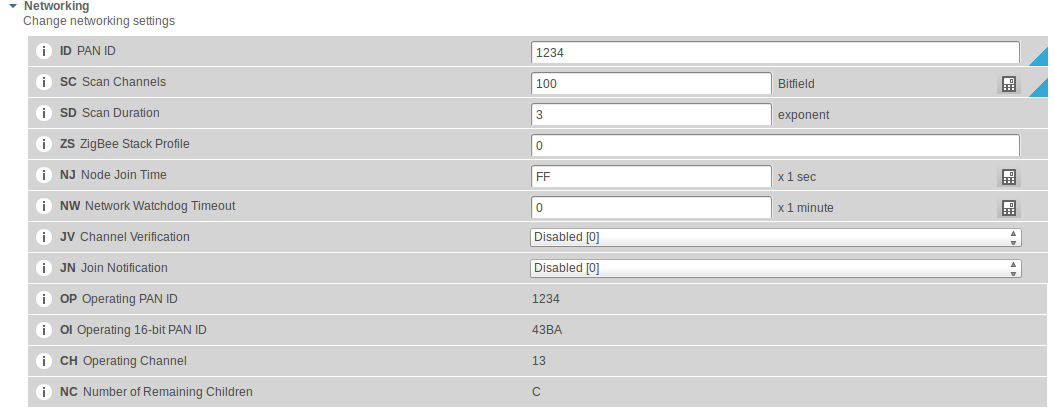
\includegraphics[width=0.9\linewidth]{Figures/XCTU/RouterNet}}
\caption{Configuraciones finales en el Router, 1.}
\label{fig:RNet}
\end{figure}

\begin{figure}[H] % Example image
\center{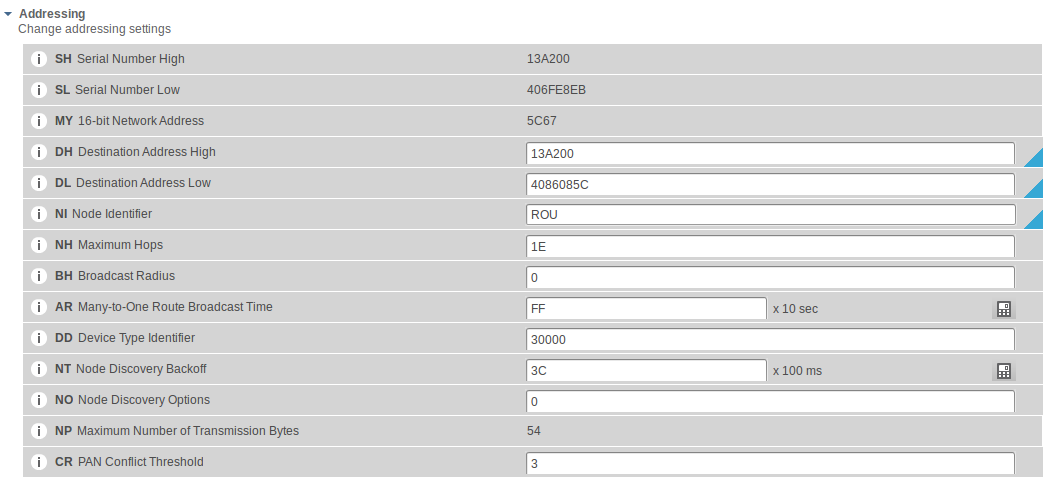
\includegraphics[width=0.9\linewidth]{Figures/XCTU/RouterAd}}
\caption{Configuraciones finales en el Router, 2.}
\label{fig:RAd}
\end{figure}

\newpage

\section{Prueba: Un chat}
\subsection{Preparativos}
Esta prueba puede realizarse utilizando el modo consola de XCTU en dos computadoras (mire la subsección \ref{subsubsec:ConCoor}, donde se explica el modo de ingresar a dicha ventana). Sin embargo, puede probar con una terminal y XCTU en una misma PC, o dos sesiones distintas de terminales. Existen diversidad de ellas en internet, que se pueden usar para evitar instalar XCTU en cada PC o dispositivo que requiera el uso de los XBEE. Una de ellas es puTTY\footnotemark, que se usará en esta guía, junto a XCTU.

\footnotetext{Descargable de \href{http://www.chiark.greenend.org.uk/~sgtatham/putty/download.html}{http://www.chiark.greenend.org.uk/~sgtatham/putty/download.html}}

PuTTY no es necesario que sea instalado como cualquier programa de Windows, ya que solo es un ejecutable que al ser invocado, pedirá inmediatamente los datos para establecer una conexión, tal y como muestra la figura \ref{fig:Pu}.

\begin{figure}[H] % Example image
\center{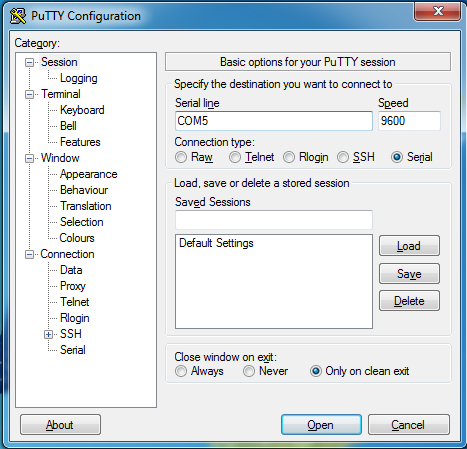
\includegraphics[width=0.7\linewidth]{Figures/XCTU/Putty}}
\caption{Configuración de sesión en PuTTY.}
\label{fig:Pu}
\end{figure}

No importa si que XBEE se elija para comunicarse con XCTU o una terminal, es indistinto. En la ventana de configuraciones de PuTTY que se abre se deberá seleccionar, en el área llamada \textit{Connection type:}, a \textbf{Serial}. Entonces, en la caja de texto de \textit{Serial line} deberá colocar el puerto a través del cual se comunica la PC con el XBEE (mire la subsección \ref{subsubsec:Iden}). En el área demominada \textit{Speed} deberá colocar la velocidad, en baudios, a la cual una PC se comunica con el XBEE. Es la misma a la cual XCTU reconoció dicho XBEE. En este caso, se trata de 9600 baudios a través del puerto COM5. El resto de la ventana se deja por defecto, ahora de clic en \textit{\textbf{Open}}. Se abrirá una ventana como la que se muestra en la figura \ref{fig:PuttCon}.

\begin{figure}[H] % Example image
\center{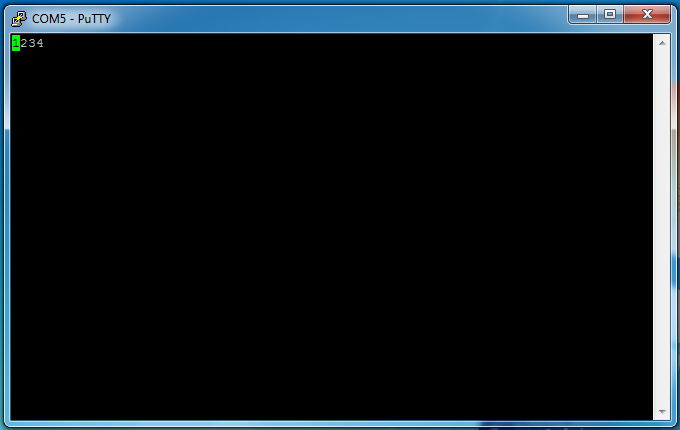
\includegraphics[width=0.7\linewidth]{Figures/XCTU/PuttyConsole}}
\caption{Terminal PuTTY.}
\label{fig:PuttCon}
\end{figure}

Para comprobar que la comunicación se estableció correctamente, teclee los tres signos de suma (\textcolor{blue}{+++}, como cuando se utilizó el modo consola de XCTU en la subsección \ref{subsubsec:ConCoor}). El XBEE deberá responder con un \textcolor{red}{OK}. De ser el caso, teclee \textcolor{blue}{ATCN} para ingresar al modo de recepción y envío de datos para estar listos para el chat. 

Para el otro XBEE, repita los pasos de apertura de consola en la subsección \ref{subsubsec:ConCoor}, dejando abierta la consola y verificando que el XBEE de respuesta al comando \textcolor{blue}{+++}, y de ser ese el caso, teclee \textcolor{blue}{ATCN}. 

\subsection{Chateando}

Proceda a teclear un texto cualquiera tanto en PuTTY como en la consola de XCTU. Lo que se escriba en la primera deberá de aparecer en la segunda, y viceversa, como se muestra en la figura \ref{fig:Fin}. Como nota, en PuTTY puede leer lo que recibe, mas no el texto que teclea y envía, a diferencia de la consola de XCTU que muestra tanto los textos de envío y recepción. 

\begin{figure}[H] % Example image
\center{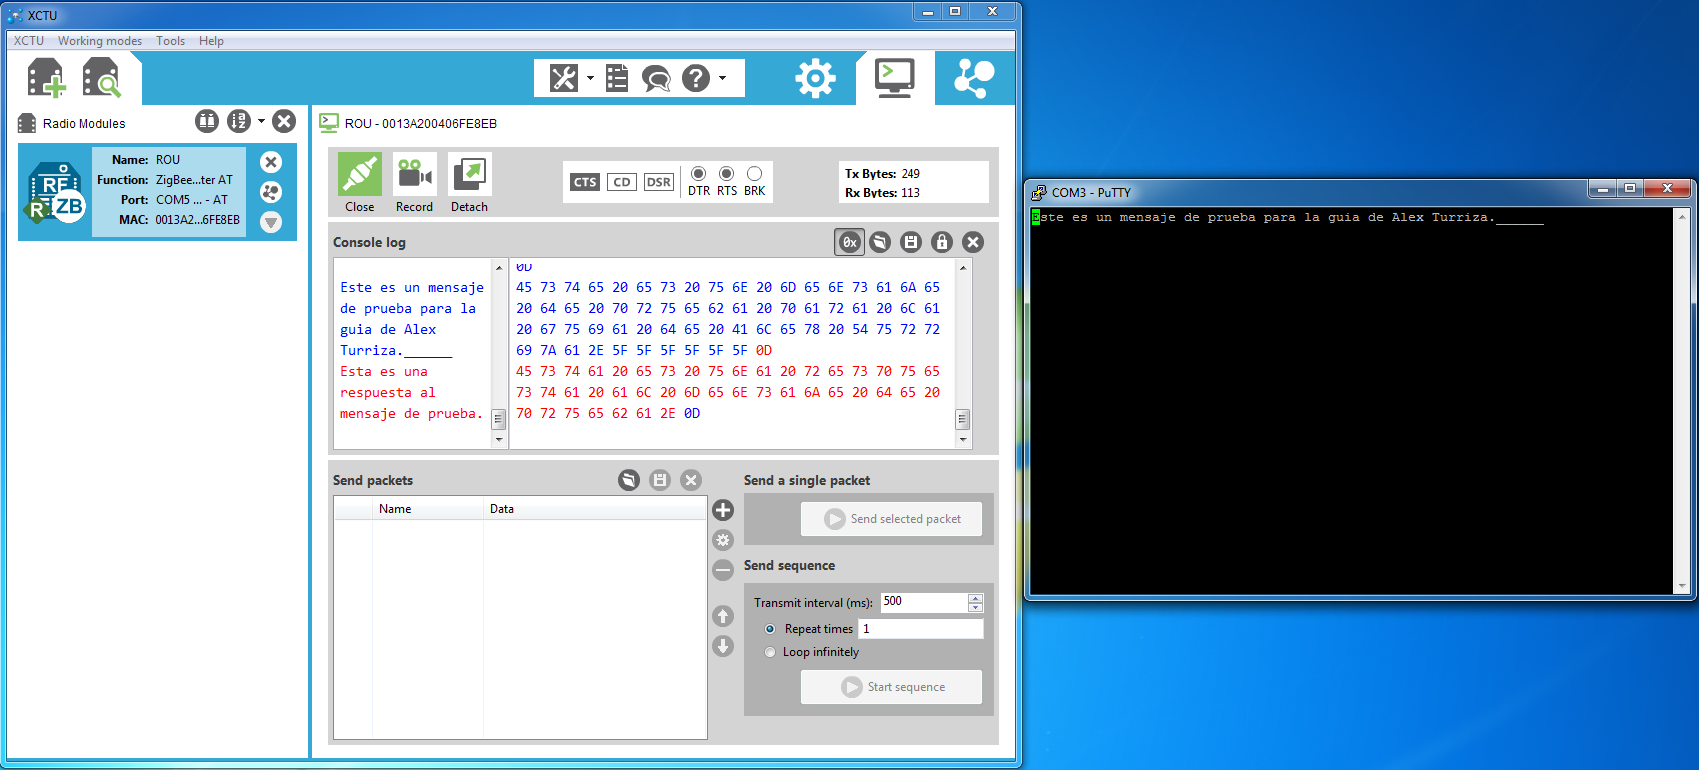
\includegraphics[width=1\linewidth]{Figures/XCTU/Final}}
\caption{El chat funcionando.}
\label{fig:Fin}
\end{figure}

Habiendo verificado que todo funcione correctamente y los XBEE estén comunicándose, ya podrán usarse en los proyectos. En caso contrario, verifique la configuración en la sección \ref{StartConf}.
%\end{document}